\section{Beschreibung des Datenbankaufbaus}
Die Datenbank des Systems Sensora ist im Schema sensora organisiert und verfolgt eine klar strukturierte, relationale Modellierung mit durchdachter Referentialität und Typisierung. Sie unterstützt die zentralen Funktionen des Systems wie Benutzerverwaltung, Gruppenzugehörigkeit, Raum- und Pflanzenzuordnung sowie Sensor- und Steuerdaten.

\begin{figure}[h]
\centering
%  \includesvg[width=\linewidth, height=0.9\textheight, keepaspectratio,inkscapelatex=false]{img/Datenbank Diagramm.svg}
  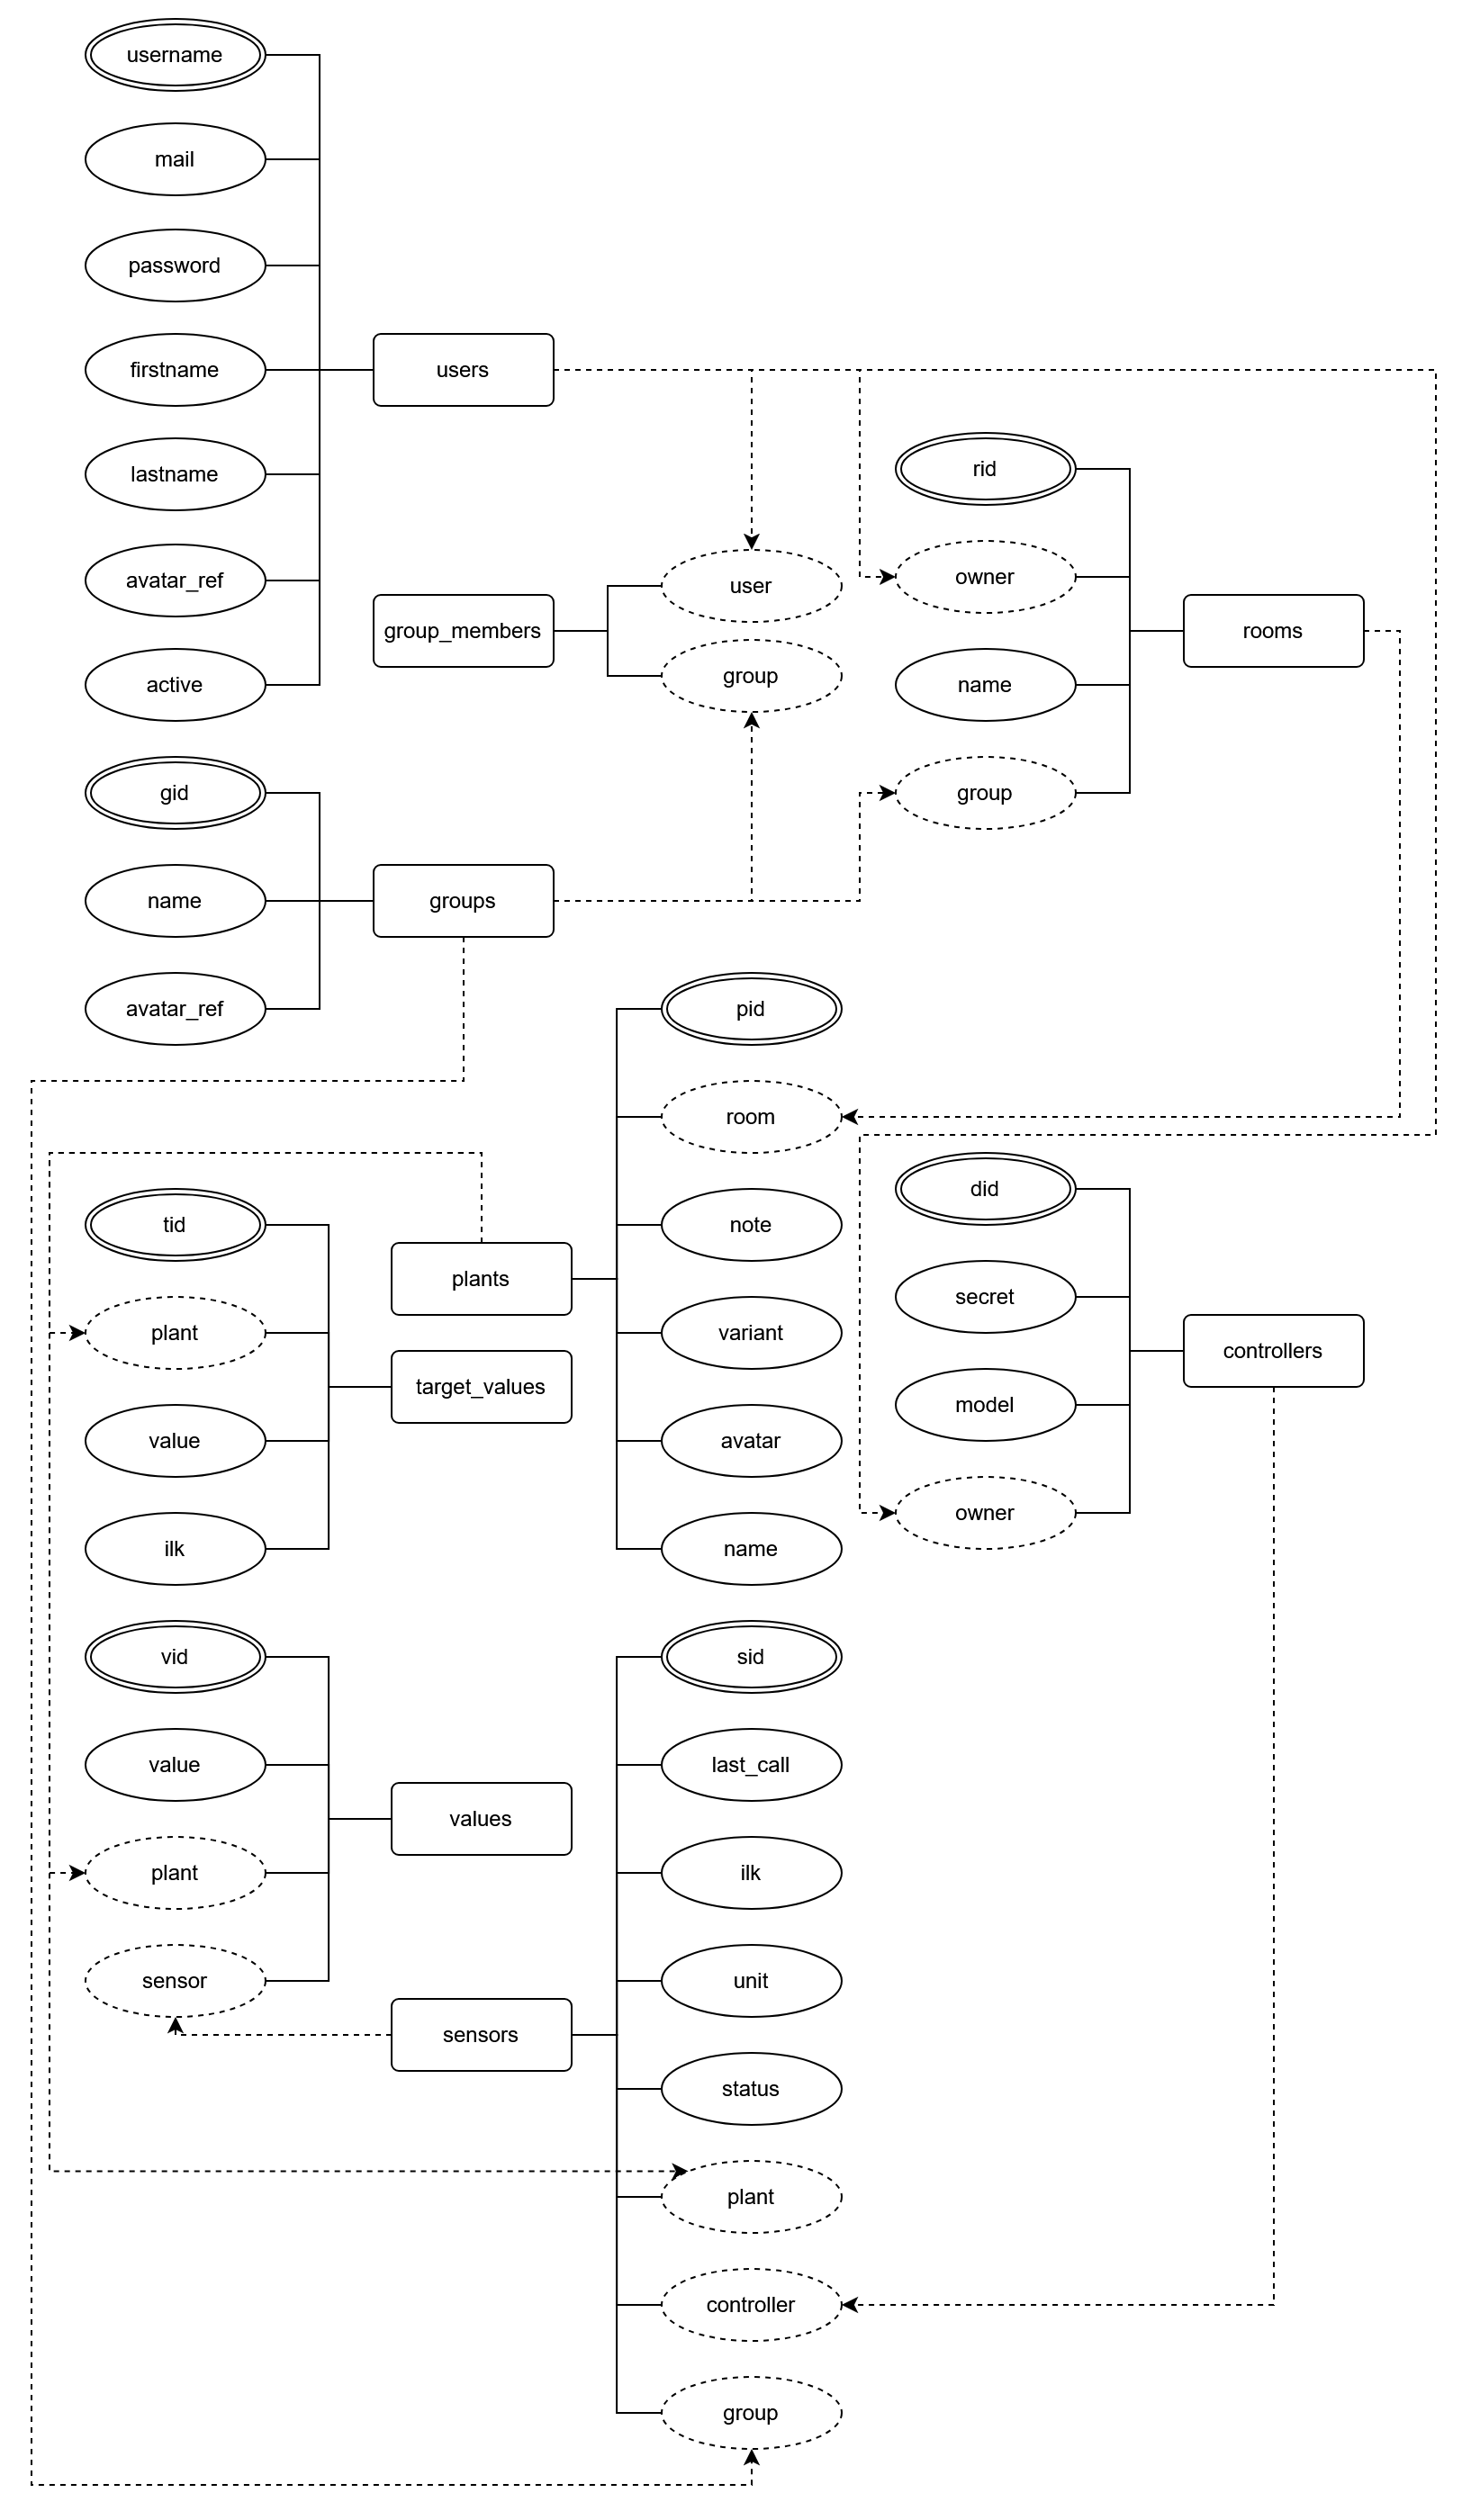
\includegraphics[width=\linewidth, height=0.9\textheight]{img/Datenbank Diagramm.png}
\caption{Sensora Datenbank Struktur}
\label{fig:sensora_datenbank}
\end{figure}

\subsection{Struktur und Besonderheiten}
\begin{description}
    \item[Benutzerverwaltung:]
    Die Tabelle users bildet die zentrale Entität für Benutzer ab. Jeder Benutzer besitzt Pflichtangaben sowie einen referenzierten Avatar aus dem dedizierten ENUM-Typ sensora.avatar. Die E-Mail-Adresse ist eindeutig.
    \item[Gruppen \& Mitgliedschaften:]
    Gruppen (groups) können mehrere Mitglieder haben, realisiert durch die Join-Tabelle group\_members. Diese bildet eine klassische Many-to-Many-Beziehung zwischen Nutzern und Gruppen ab.
    \item[Räume \& Pflanzen:]
    Räume (rooms) können Gruppen zugeordnet sein und besitzen jeweils einen Eigentümer. Pflanzen (plants) sind immer einem Raum zugeordnet und dienen als Ankerpunkt für Messwerte.
    \item [Sensorik \& Steuerung:]
    Sensoren (sensors) sind mit Controllern (controllers) verknüpft und optional direkt mit einer Pflanze oder Gruppe verbunden. Jeder Sensor verwendet den ENUM-Typ sensora.status, um seinen Zustand zu klassifizieren.
    \item [Zielwerte \& Messdaten:]
    Pflanzen können über target\_values Zielgrößen definieren. Tatsächliche Messwerte werden in der Tabelle values gespeichert und jeweils einem Sensor sowie einer Pflanze zugeordnet.
\end{description}

\subsection{Technische Merkmale}
\begin{itemize}
    \item Es kommen ENUM-Typen zum Einsatz, um Felder wie Avatar und Status typensicher und standardisiert zu definieren.
    \item Sämtliche Fremdschlüsselbeziehungen nutzen CASCADE-Strategien zur Pflege von Konsistenz (z.B. beim Löschen von Benutzern oder Pflanzen).
    \item Indizes auf eindeutige Felder (z.B. mail, secret) erhöhen die Performanz gezielter Abfragen.
    \item Die Nutzung von Timestamps mit Standardwerten erlaubt eine automatische Protokollierung von Ereignissen wie Sensoraktivität.
\end{itemize}

Diese Datenbankstruktur ermöglicht eine flexible, erweiterbare und gleichzeitig robuste Grundlage für die Backend-Logik und garantiert eine nachvollziehbare Abbildung der fachlichen Entitäten.